\documentclass[12pt]{article}

\usepackage{graphicx}

\title{Overview of SMART Mobility Urban Science Pillar task 2.2.2.2018: Coupling Land Use Models and Network Flow Models}

\date{January 2018}

\begin{document}
	
\maketitle

Integrating land use, travel demand, and traffic models represents a gold standard for regional planning, but is rarely achieved in a meaningful way, especially at the scale of disaggregate data. This project develops a new pipeline architecture for integrated modeling of urban land use, travel demand, and traffic assignment (Figure \ref{fig:overview_pipeline_architecture}). Our land use model, UrbanSim, is an open-source microsimulation platform used by metropolitan planning organizations worldwide for modeling the growth and development of cities over long ($\sim$30 year) time horizons. UrbanSim is particularly powerful as a scenario analysis tool, enabling planners to compare and contrast the impacts of different policy decisions on long term land use forecasts in a statistically rigorous way. Our travel demand model, ActivitySim, is an agent-based modeling platform that produces synthetic origin--destination travel demand data. Finally, we use a static user equilibrium traffic assignment model based on the Frank-Wolfe algorithm to assign vehicles to specific network paths to make trips between origins and destinations. This traffic assignment model runs in a high-performance computing environment. The resulting congested travel time data can then be fed back into UrbanSim and ActivitySim for the next model run.

In this preliminary phase of the project, we have recently completed an integration of our land use model (UrbanSim) and travel demand model (ActivitySim), which marks a first for urban microsimulation. We are constructing graph models of metropolitan-scale road networks on-demand, with configurable resolution (that is, tertiary roads and up, or all drivable roads if desired). Finally, we recently completed a preliminary hand-off of our synthetic travel demand data to a static user equilibrium traffic assignment model in an HPC environment, with a successful test model run.

This ongoing effort will focus on adding workplace choice and vehicle ownership into the UrbanSim models and tightly integrating this with network models. With the behaviorally integrated models and a sufficiently detailed representation of the transportation network and geography, ideally using local streets and parcels and buildings, we will be able to explore the long-term feedback effects of transportation infrastructure changes on urban development patterns. We will be able to include the feedback effects of these urban development dynamics on travel demand and on travel flows and speeds, and consequently on transportation-related energy consumption.

\begin{figure}[htbp]
	\center
	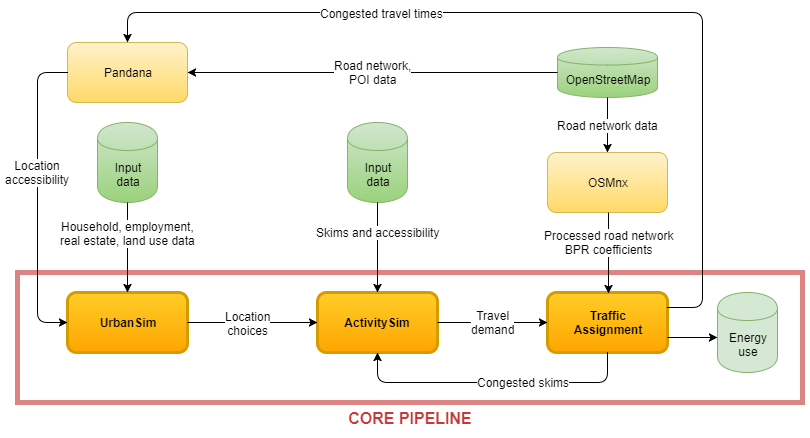
\includegraphics[width=\textwidth]{diagram_pipeline.png}
	\caption{Overview of the integrated modeling pipeline's architecture}
	\label{fig:overview_pipeline_architecture}
\end{figure}

This project has four key deliverables due to the Department of Energy over FY18. Our Q1 deliverable (completed) is a technical report on the progress so far and the preliminary architecture of this integrated modeling pipeline. The Q2 deliverable is a network flow model running at scale, integrated with UrbanSim and ActivitySim. The Q3 deliverable is a journal article manuscript describing these accomplishments, to be submitted for peer review. Finally, the Q4 deliverable is a code repository for this code to run at scale.

\end{document}